\documentclass[11pt,a4paper]{article}

\usepackage[T1]{fontenc}
\usepackage[utf8]{inputenc}
\usepackage{mathptmx}
\usepackage{courier}
\usepackage[margin=2.5cm]{geometry}
\usepackage{amsmath}
\usepackage{booktabs}
\usepackage{graphicx}
\usepackage{xcolor}
\usepackage[numbers,sort&compress]{natbib}
\usepackage{xurl}
\usepackage[hidelinks]{hyperref}
\hypersetup{pdftitle={Small Convolutional Networks for PTB-XL Superclasses: A Five-Seed Comparison with Patient-Level Intervals and Selective Prediction},pdfauthor={Muzammal Hussain}}
\usepackage{caption}
\captionsetup{font=small,labelfont=bf}

\newcommand{\code}[1]{\texttt{#1}}
\setlength{\emergencystretch}{3em}

\title{\textbf{Small Convolutional Networks for PTB-XL Superclasses:\\A Five-Seed Comparison with Patient-Level Intervals\\and Selective Prediction}}
\author{Muzammal Hussain\\
\small Independent researcher, Glasgow, United Kingdom\\
\small \href{mailto:muzammal@masmatixinnovations.co.uk}{muzammal@masmatixinnovations.co.uk}\\
\small ORCID: \href{https://orcid.org/0009-0001-2570-5686}{0009-0001-2570-5686}}
\date{\small November 2026}

\begin{document}
\maketitle

\begin{abstract}
\noindent
Results on PTB-XL are often reported from a single training run, without an interval and without saying how the
model behaves when it is unsure. We train two compact 1D networks, a plain convolutional network (76k parameters)
and a residual network (195k parameters), on the five diagnostic superclasses of PTB-XL 1.0.3 at 100\,Hz, with the
recommended patient-disjoint folds (17,084 training, 2,146 validation and 2,158 test records). Each model is
trained with five seeds; decision thresholds are chosen on the validation fold only, and intervals come from 1,000
patient-level bootstrap resamples of the test fold. The residual network reaches macro AUROC
$0.925 \pm 0.003$ over seeds against $0.918 \pm 0.002$ for the plain network; averaging the five seeds gives 0.932
[0.924, 0.939] and 0.923 [0.915, 0.930]. The paired difference of the seed ensembles is $+0.009$ [$+0.007$, $+0.011$],
and the residual network is ahead in four of five seeds, so the gain is small but not an accident of one seed.
Hypertrophy (HYP) is the hardest class for both models (AUROC 0.90, average precision 0.67). When the least
confident records are set aside, macro F1 of the residual ensemble rises from 0.757 on all records to 0.784 on the
most confident 80\% and 0.807 on the most confident half. The residual network matches the macro AUROC reported for
the widely used \code{resnet1d\_wang} baseline with less than half its parameters. We release the code, per-seed metrics, a Kaggle notebook
and the trained model with its normalisation statistics and thresholds.
\end{abstract}

\section{Introduction}

PTB-XL \citep{wagner2020ptbxl} is the largest openly licensed collection of clinical 12-lead ECGs with
cardiologist-annotated statements, and its five diagnostic superclasses (normal ECG, myocardial infarction,
ST/T change, conduction disturbance and hypertrophy) have become a standard multi-label task. The benchmark of
\citet{strodthoff2021benchmarks} fixed the evaluation: the dataset's ten stratified, patient-disjoint folds, with
fold 9 for validation and fold 10 for testing, and macro AUROC as the main score. Their best convolutional and
recurrent models reach macro AUROC of about 0.93 on the diagnostic tasks.

Two things are often missing when a new result is added to this line of work. First, a single run says little:
differences of 0.005 AUROC between architectures are within the spread caused by the random seed. Second, a
macro AUROC does not tell a user what happens at a fixed threshold, or whether the model knows when it is likely
to be wrong. This paper asks three narrow questions about small models that fit on any laptop:

\begin{enumerate}
\item Does a residual 1D network beat a plain 1D network of the same width once seed variation and
patient-level uncertainty are counted?
\item Which superclasses remain hard for both?
\item How much does macro F1 improve if the model is allowed to set aside its least confident records?
\end{enumerate}

\noindent The contributions are a five-seed comparison with patient-level bootstrap intervals and a paired
difference; per-class results showing where the errors sit; a selective-prediction curve with thresholds fixed on
validation data; and a released, reproducible package (code, Kaggle notebook, per-seed outputs and a model card).

\section{Related work}

\citet{strodthoff2021benchmarks} compared convolutional, recurrent and wavelet-feature models on all PTB-XL tasks
and found that residual and Inception-style 1D networks were strongest. Their \code{resnet1d\_wang} adapts the
fully convolutional time-series baseline of \citet{wang2017tsc}, and \code{xresnet1d101} follows the residual design
of \citet{he2016resnet}. A recent re-run of these baselines with repeated training reports superclass macro AUROC
of 0.9253 (SD 0.003) for \code{resnet1d\_wang} with 451k parameters and 0.9148 (SD 0.002) for
\code{xresnet1d101} with 1.88M parameters \citep{abreu2025code2}. Selective classification, in which a model may
abstain and is judged on the records it keeps, was formalised for deep networks by
\citet{geifman2017selective}; we use a simple confidence score rather than a learned rejection head.

\section{Data and setup}

\paragraph{Data.} We use PTB-XL version 1.0.3 at 100\,Hz (12 leads, 10\,s, 1,000 samples per lead). Each diagnostic
SCP statement of a record is mapped to its \code{diagnostic\_class}; a record is kept if it has at least one of the
five superclasses, which leaves 21,388 of the 21,799 records. Folds 1--8 form the training set (17,084 records), fold 9
the validation set (2,146) and fold 10 the test set (2,158); the code checks that no patient appears in more than one
split. Each lead is standardised with the mean and standard deviation of the training folds only. The data are
downloaded from PhysioNet at run time and checked against the published SHA-256 sums; nothing is re-hosted.

\paragraph{Models.} Both networks take a $12 \times 1000$ input and use the widths (32, 64, 128), global average
pooling, dropout 0.2 and a linear layer with five outputs. The plain network has three blocks of a kernel-7
convolution, batch normalisation, ReLU and max pooling (75,685 parameters). The residual network has three blocks of
two convolutions (kernels 7 and 5) with batch normalisation and a shortcut, the last two with stride 2 (194,501
parameters).

\paragraph{Training.} We minimise binary cross-entropy with AdamW \citep{loshchilov2019adamw} (learning rate
$10^{-3}$, weight decay $10^{-4}$, batch size 32) for at most 40 epochs, stopping when the validation loss has not
improved for 5 epochs and keeping the best checkpoint. Each model is trained with seeds 17, 23, 31, 47 and 59 on
one Kaggle GPU; a run takes 0.5--1.7 minutes and stops after 11--20 epochs.

\paragraph{Evaluation.} Macro AUROC over the five classes on the test fold is the main score, with average
precision per class. For F1, each class gets its own threshold, chosen from $\{0.10, 0.15, \dots, 0.90\}$ to maximise
F1 on the validation fold. The seed ensemble averages the five seeds' probabilities and uses the mean of their
thresholds. Intervals are 95\% percentile intervals from 1,000 bootstrap resamples of test patients, so that all
records of one patient move together; the ResNet$-$CNN difference is computed on the same resamples. For selective
prediction, the confidence of a record is the mean over classes of $\max(p, 1-p)$; we keep the most confident
100\% to 50\% of test records and report macro F1 on the kept records.

\section{Results}

\begin{table}[t]
\centering
\caption{Test results on PTB-XL fold 10 (2,158 records). Mean $\pm$ SD over five seeds; ensemble = mean of the five
seeds' probabilities, with 95\% patient-level bootstrap intervals. Macro F1 uses validation thresholds.}
\label{tab:main}
\small
\begin{tabular}{lcccc}
\toprule
Model & Params & Macro AUROC & Ensemble macro AUROC & Ensemble macro F1 at 100 / 80 / 50\% kept \\
\midrule
1D CNN    & 76k  & $0.9184 \pm 0.0022$ & 0.9227 [0.9148, 0.9305] & 0.748 / 0.770 / 0.794 \\
1D ResNet & 195k & $0.9250 \pm 0.0030$ & 0.9317 [0.9242, 0.9387] & 0.757 / 0.784 / 0.807 \\
\midrule
\multicolumn{5}{l}{ResNet $-$ CNN (ensembles): $+0.0090$ [$+0.0068$, $+0.0113$]; ResNet higher in 4 of 5 paired seeds.}\\
\bottomrule
\end{tabular}
\end{table}

\paragraph{Residual versus plain.} Table~\ref{tab:main} gives the main numbers. Per seed, the residual network
ranges from 0.920 to 0.928 and the plain network from 0.916 to 0.921; the ranges overlap, and the one seed where
the plain network is ahead (seed 59) shows why a single run could point either way. Averaged over seeds, and
paired on the same bootstrap resamples, the residual network is better by 0.009 AUROC with an interval that excludes
zero. The mean macro F1 of single runs is 0.745 for the residual and 0.736 for the plain network; ensembling adds
about 0.01 to both. The residual network's mean single-run AUROC (0.925) matches the 0.9253 reported for
\code{resnet1d\_wang} \citep{abreu2025code2} with fewer than half its parameters, although that figure comes
from a different training pipeline and is not a paired comparison.

\begin{table}[t]
\centering
\caption{Per-class test AUROC and average precision (AP), mean over five seeds.}
\label{tab:labels}
\small
\begin{tabular}{lccccc}
\toprule
 & NORM & MI & STTC & CD & HYP \\
\midrule
AUROC, 1D CNN    & 0.938 & 0.915 & 0.933 & 0.912 & 0.894 \\
AUROC, 1D ResNet & 0.945 & 0.927 & 0.933 & 0.919 & 0.902 \\
AP, 1D CNN       & 0.915 & 0.813 & 0.821 & 0.830 & 0.664 \\
AP, 1D ResNet    & 0.924 & 0.835 & 0.824 & 0.842 & 0.672 \\
\bottomrule
\end{tabular}
\end{table}

\paragraph{Where the errors are.} Table~\ref{tab:labels} shows that the residual network's gain comes mainly from
myocardial infarction (+0.012 AUROC, +0.022 AP) and conduction disturbance; on ST/T change the two are equal.
Hypertrophy is the weakest class for both, with AP near 0.67, well below the other four. Hypertrophy is the rarest
superclass in PTB-XL \citep{wagner2020ptbxl}, and it is the class where a small model should be trusted least.

\begin{figure}[t]
\centering
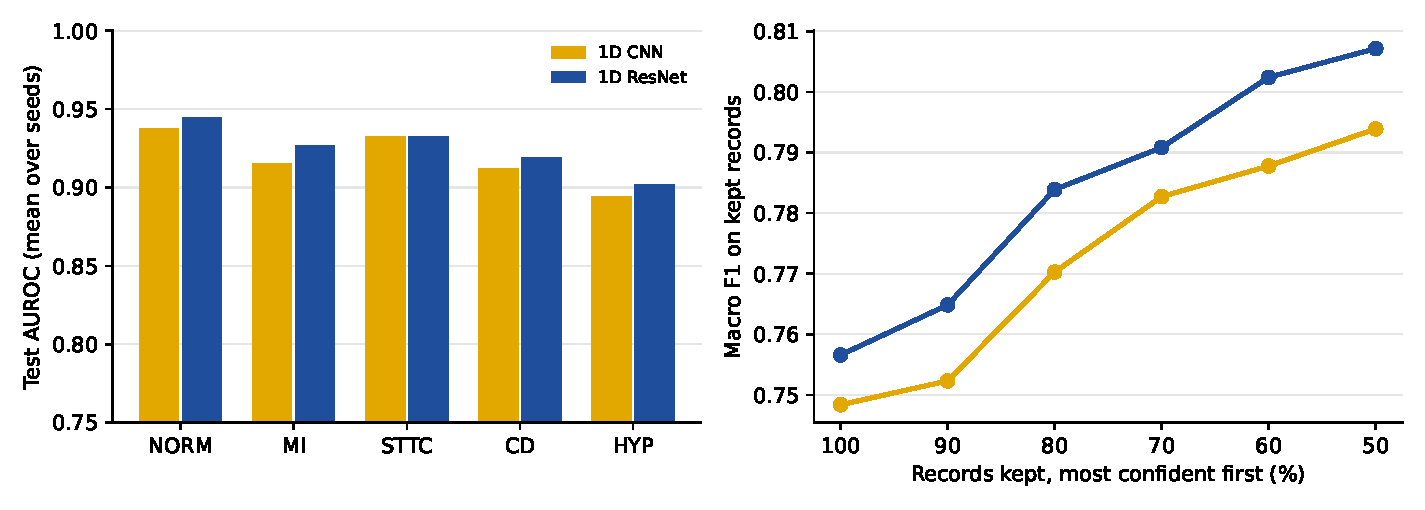
\includegraphics[width=\linewidth]{figures/fig_auroc_selective.pdf}
\caption{Left: per-class test AUROC, mean over five seeds. Right: macro F1 of the seed ensembles on the most
confident share of test records (validation thresholds).}
\label{fig:main}
\end{figure}

\paragraph{Selective prediction.} Figure~\ref{fig:main} (right) shows macro F1 as the least confident records are
set aside. For the residual ensemble it rises from 0.757 on all records to 0.765 at 90\%, 0.784 at 80\% and 0.807 at
50\%; the plain ensemble follows the same shape about 0.01 lower. With a fixed cut-off of 0.8 on the confidence
score, single residual runs keep on average 87\% of test records (84\% for the plain network). The gain from
abstaining (about 0.05 macro F1 at half coverage) is real but modest: low confidence flags some of the errors, not
most of them.

\section{Limitations}

All results come from one dataset, one test fold and one acquisition site, so they say nothing about other
hospitals or devices. Labels are the five superclasses, which hide large differences within each class. The
confidence score is a heuristic, not a calibrated probability of error, and the selective-prediction curve is not a
clinical safety guarantee. The residual network also has more parameters than the plain one (195k against 76k), so the comparison does not
separate the effect of the shortcuts from that of size. We did not tune hyperparameters beyond the fixed setting above, and the comparison with
published baselines is unpaired. The models are research artefacts and are not intended for diagnosis.

\section{Conclusion}

With five seeds and patient-level intervals, a 195k-parameter residual 1D network is better than a plain network of
the same width by a small but consistent 0.009 macro AUROC on the PTB-XL superclasses, and reaches the level of
much larger published baselines. Hypertrophy remains the weak class, and letting the model abstain on its least
confident half raises macro F1 by about 0.05. We suggest that new PTB-XL results report several seeds, patient-level
intervals and a selective-prediction curve alongside the usual macro AUROC.

\section*{Code and data availability}

Code, the Kaggle notebook, per-seed metrics and the analysis files are at
\url{https://github.com/MHKhan50/ptbxl-ecg-superclass-benchmark}, archived at
\href{https://doi.org/10.5281/zenodo.24407647}{doi:10.5281/zenodo.24407647}. The trained residual network (seed 23, lowest
validation loss), with its normalisation statistics, thresholds and model card, is at
\url{https://huggingface.co/MHkhan50/ptbxl-ecg-resnet}. PTB-XL is available from PhysioNet under CC BY 4.0
\citep{wagner2020ptbxl}.

\bibliographystyle{plainnat}
\bibliography{references}

\end{document}
